% =====================================================================
% Appendix: supplementary results and figures
%
% Collects result tables and figures produced by the analysis code but not
% reproduced in the main chapters, grouped by the chapter they support.
%
% Placement: after the last chapter of the main matter. \appendix must appear
% exactly once in the document -- if it is already declared elsewhere, delete
% the \appendix line below. If the thesis class has no \chapter (e.g. article),
% demote \chapter -> \section and each \section -> \subsection.
%
% Figures live under docs/images/ in the repository and are expected under
% images/ in the thesis tree. They are exported at their final printed width
% and must be included with width=\linewidth without further scaling.
%
% Editorial rule applied here: every table or figure keeps a self-contained
% caption that states what is reported and how to read the encoding, plus one
% short paragraph giving the fact it supports and the place in the main text
% where that fact is used. Material that cannot be read without the main text
% does not belong in an appendix, and an appendix of bare outputs cannot be
% assessed.
% =====================================================================
\chapter{Supplementary results and figures}
\label{app:figures}

This appendix collects the result tables and figures produced during the
analysis that are not reproduced in the main chapters. They are included for
completeness and reproducibility: each was generated by the same code and from
the same data as the corresponding main-text material, and each is referenced
from the chapter it belongs to. Material appears here rather than in the main
text when it is redundant with another table or figure, when it supports a
statement that a single number already conveys, or when it is qualitative and
therefore cannot carry an argument on its own. Nothing in this appendix is
required to follow the main line of reasoning.


\section{Datasets}
\label{app:figures_datasets}

The four figures below complement Section~\ref{sec:dataset_analysis}. All are produced by the dataset analysis notebook from the same adapters used at training time, so split sizes, class indices, and hierarchy edges are identical to those seen by the models. As in the main text, they are descriptive: they characterize the data and the label space, not the behaviour of any model.

\subsection{Split sizes and composition}

Figure~\ref{fig:app_split_composition} shows the same partition reported numerically in Table~\ref{tab:protocol_splits}. It is kept out of the main text because nine numbers are read more precisely from the table than from a bar chart, but the percentage panel makes one asymmetry immediate: CIFAR-100 devotes 75\% of its images to training and only 8\% to validation, CUB-200-2011 44\% and 7\%, whereas the official FGVC-Aircraft partition splits the dataset into equal thirds. Model selection is therefore performed on very differently sized validation sets across the three benchmarks.

\begin{figure}[ht]
\centering
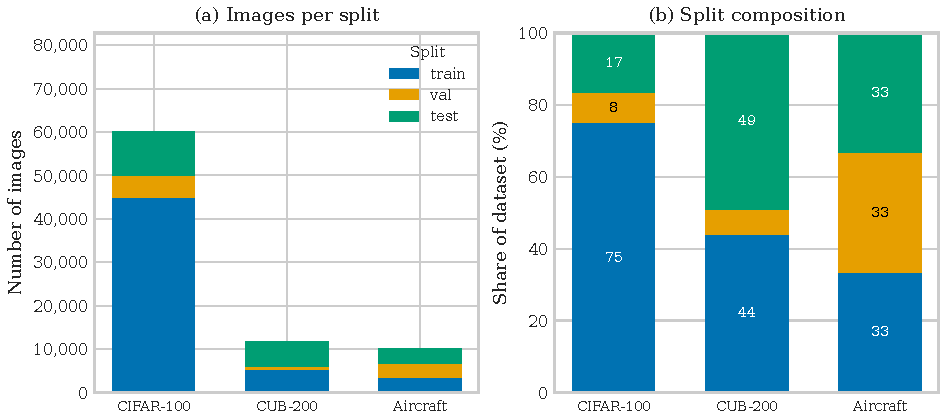
\includegraphics[width=\linewidth]{images/dataset/dataset_scale_and_taxonomy_width.pdf}
\caption{Unified-protocol split sizes. Panel (a) shows image counts and panel
(b) the corresponding train, validation and test percentages.}
\label{fig:app_split_composition}
\end{figure}

\subsection{Distribution of the branching factor}

Table~\ref{tab:branching} reports the median, maximum, and number of single-child parents of each transition; Figure~\ref{fig:app_branching} shows the full distribution behind those summaries. It confirms that the summary statistics are not hiding a different shape: the CUB family-to-species transition is genuinely long-tailed, with most families holding one to four species and a single family holding thirty, while the FGVC-Aircraft family-to-variant transition is concentrated almost entirely on one child per parent. The CIFAR-100 lower transition appears as a single horizontal line at five, since every superclass contains exactly five fine classes.

\begin{figure}[ht]
\centering
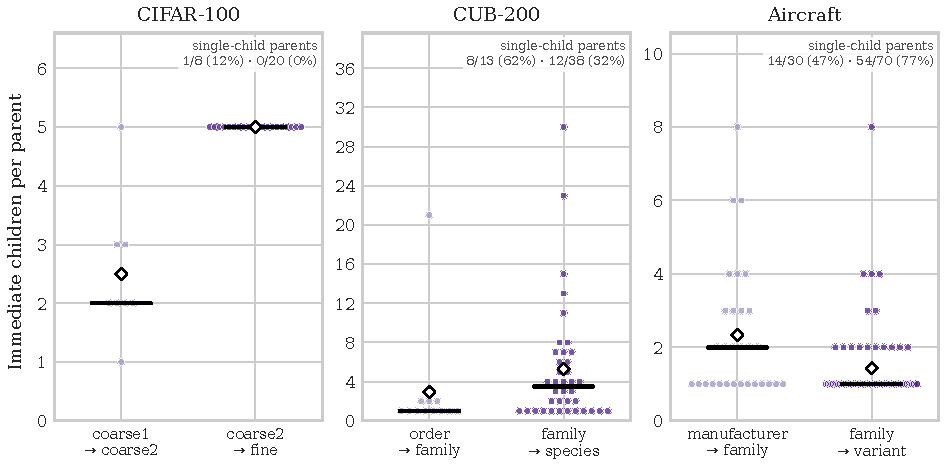
\includegraphics[width=\linewidth]{images/dataset/hierarchy_branching_beeswarms.pdf}
\caption{Distribution of children per parent at both taxonomy transitions.
Circles are parent classes; the black segment is the median, the white diamond
the mean, and annotations count single-child parents.}
\label{fig:app_branching}
\end{figure}

\subsection{Leaf classes covered by each top-level class}

Figure~\ref{fig:app_descendants} quantifies per class what the top band of the icicle plot (Figure~\ref{fig:taxonomy_icicle}) shows as areas. It is the more precise of the two views and the less immediate one, which is why the icicle is used in the main text. It makes the imbalance of the CUB taxonomy explicit: the largest order covers 133 of the 200 species and the second 23, after which every remaining order covers seven or fewer. CIFAR-100 decays gently from 25 to 5 fine classes per coarse-1 group, and FGVC-Aircraft from 22 to 1 variant per manufacturer, with 13 of its 30 manufacturers covering a single variant.

\begin{figure}[ht]
\centering
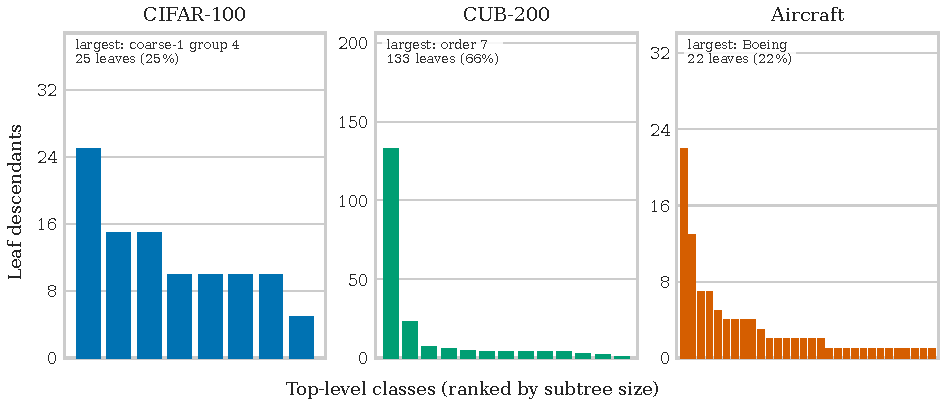
\includegraphics[width=\linewidth]{images/dataset/leaf_descendants_per_root.pdf}
\caption{Leaf classes beneath each top-level class. Bars are ranked by subtree
size within each dataset; annotations identify the largest subtree and its
share.}
\label{fig:app_descendants}
\end{figure}

\subsection{Representative images}

Figure~\ref{fig:app_gallery} is qualitative and is included only to make the difference in visual regime concrete. It illustrates why the three benchmarks are not interchangeable: CIFAR-100 classes are recognizable from coarse colour and shape at $32\times32$, whereas distinguishing two CUB species or two Aircraft variants depends on localized detail --- plumage patterning, engine count and placement, tail geometry --- that survives only at higher resolution. It does not measure visual diversity, inter-class similarity, background bias, or intrinsic difficulty, and no claim in this work rests on it.

\begin{figure}[ht]
\centering
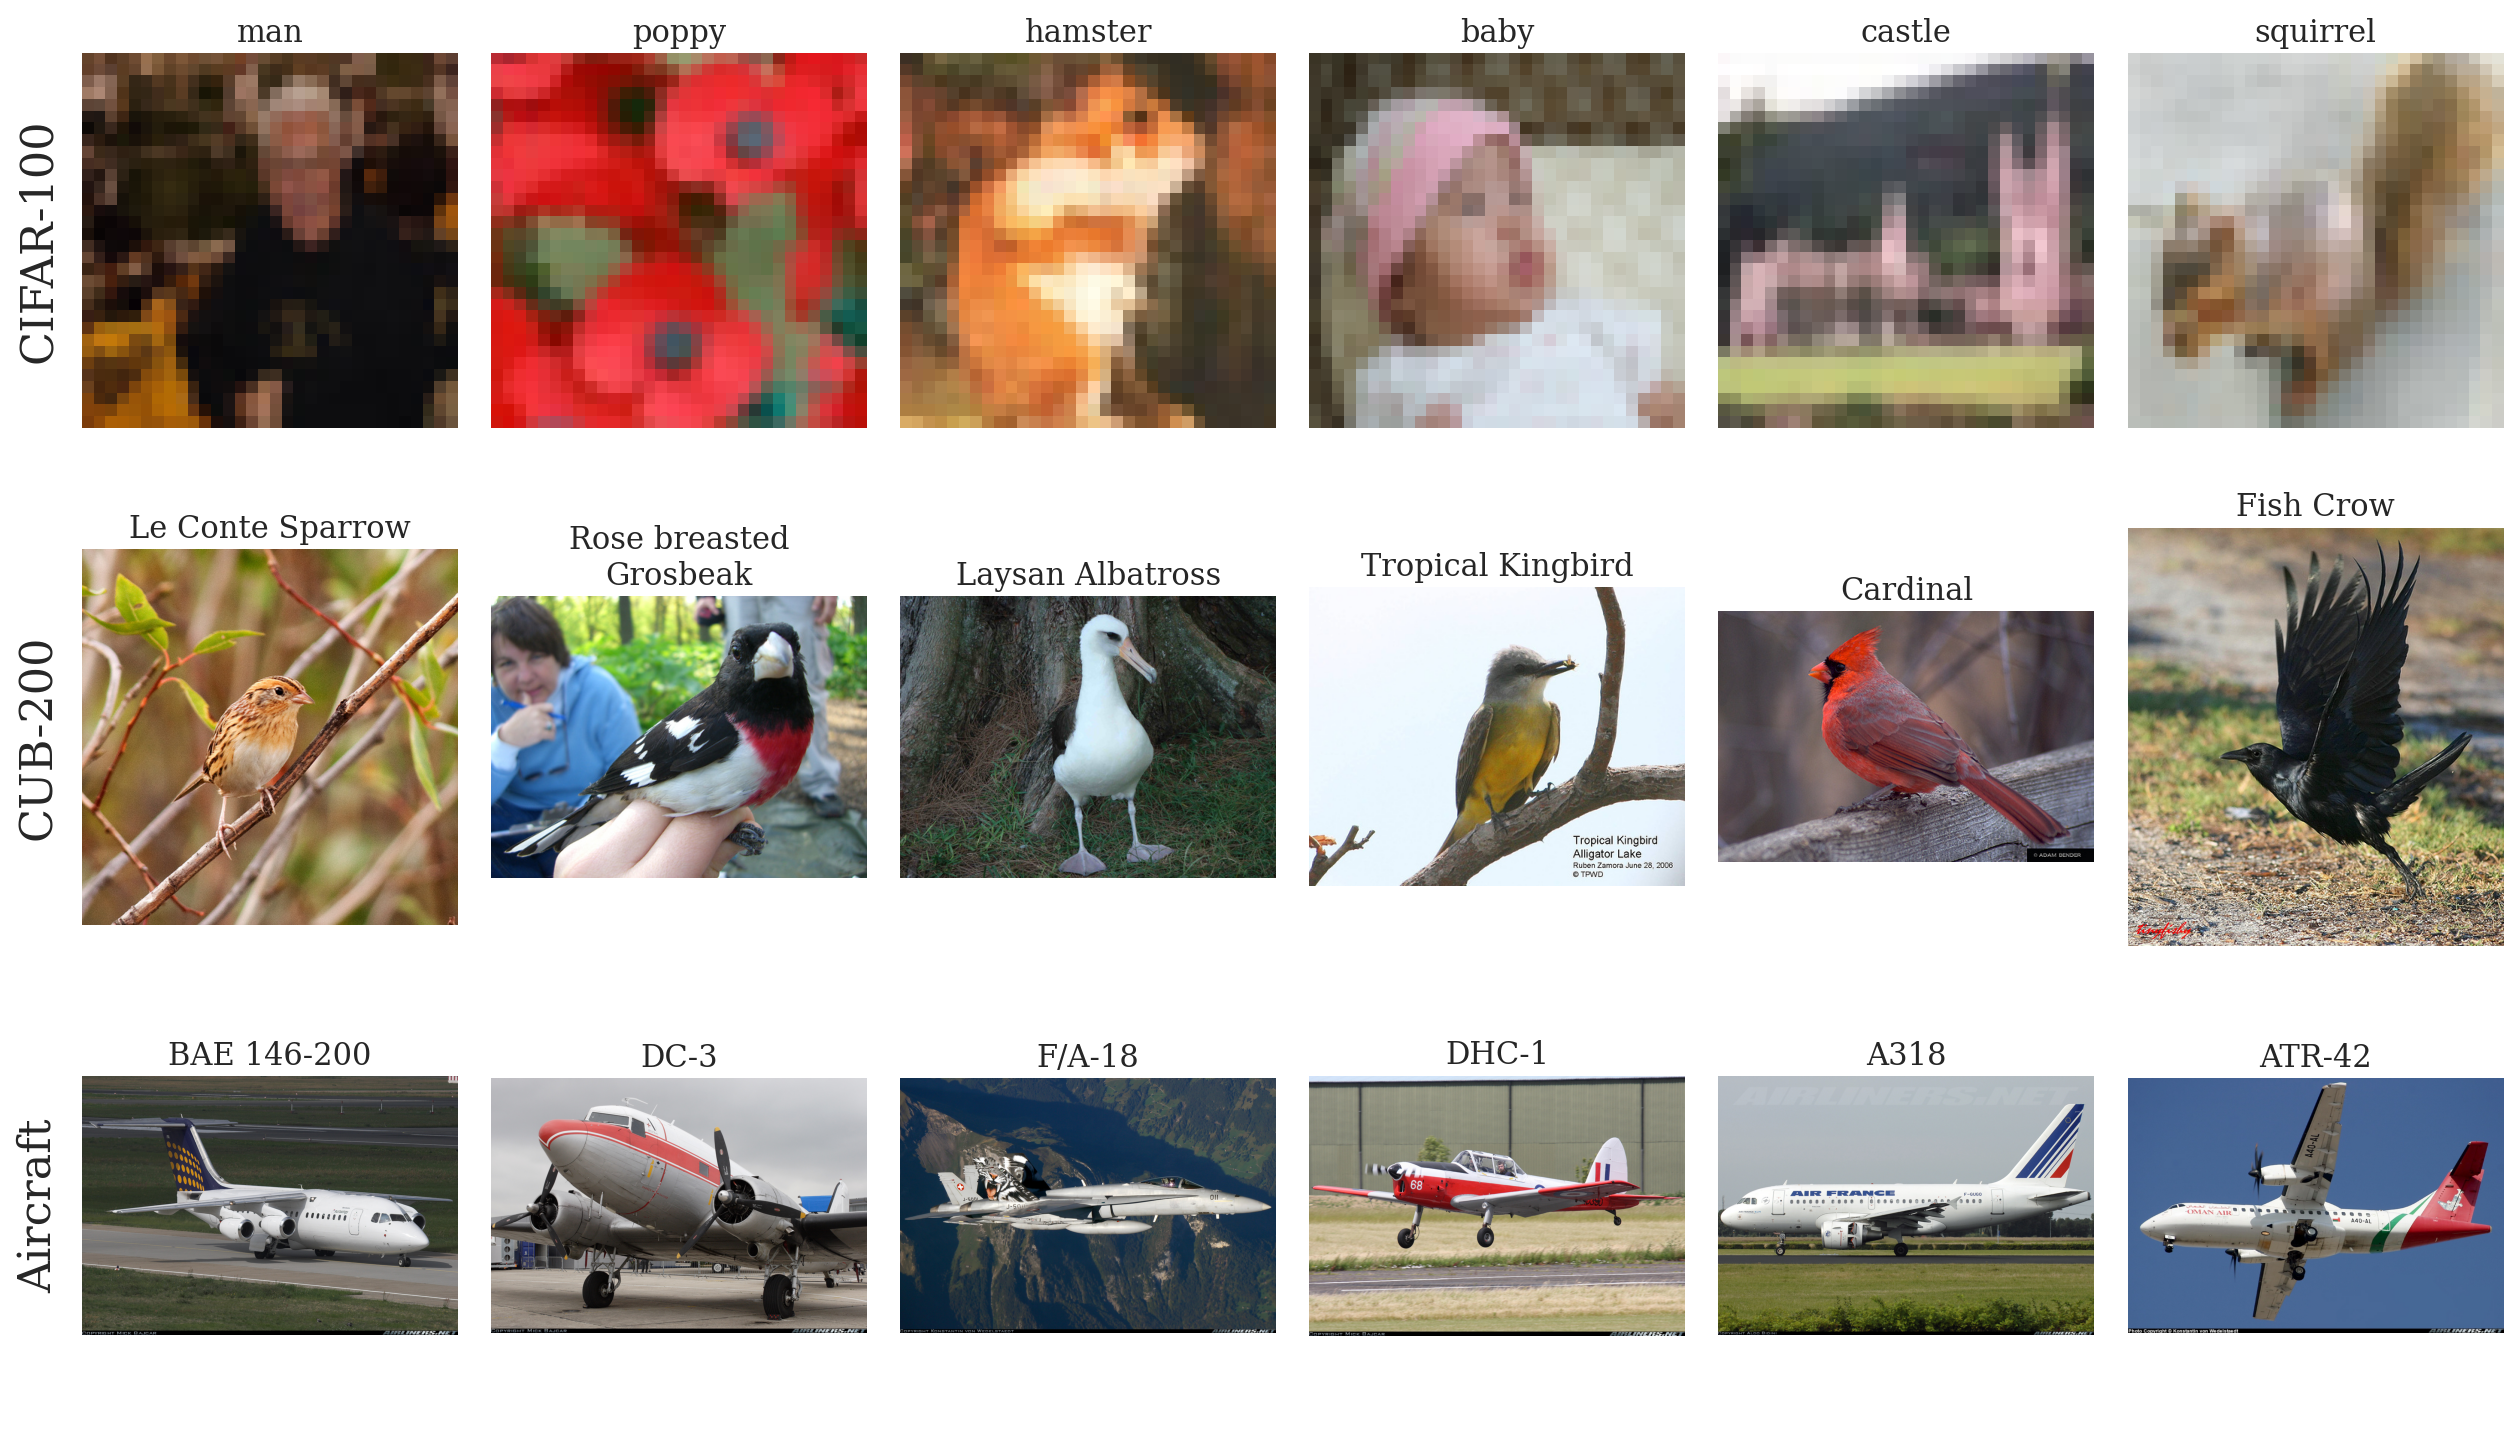
\includegraphics[width=\linewidth]{images/dataset/representative_dataset_images.png}
\caption{Fixed-seed sample of six leaf classes per dataset. Images retain their
native aspect ratio; columns do not represent related classes across rows.}
\label{fig:app_gallery}
\end{figure}

\section{Supplementary baseline results}
\label{app:figures_baselines}

\subsection{Baseline configurations}
\label{app:baseline_configs}

\Cref{tab:app_baseline_configs} summarises the effective configurations of the
fifteen baselines reported in \cref{sec:results_baselines}. These are the
launcher-resolved experimental settings, which differ in two important cases
from the defaults of the base YAML files: HRN uses the native-equivalent
\texttt{level\_conditional} decomposition, and Hier-COS uses
\texttt{global\_softmax\_ce\_reg} with \texttt{kl\_leaf} weights and a dense
random orthonormal frame. Dataset splits and checkpoint selection are common and
are therefore not repeated in the table. HCC, direct subspace supervision and
explicit lexicographic optimisation are inactive in every row; the optional
LH-projection is also inactive, while LH-DNN retains its native projection. The
complete configurations, including
normalisation constants and data-loader settings, and the commands that apply
the baseline overrides are available in the
\href{https://github.com/Gianma23/lexicographic_deep_learning_detailed_study}{project repository}.

\begin{table}[p]
\centering
\caption{Effective parameters of the reported baselines. LR is the optimiser
learning rate; the H-CAST values are the effective rates after batch-size
scaling. ``Drop'' and ``keep'' state whether the final incomplete training batch
is discarded; every validation and test batch is retained. Augmentation entries
describe the training transform. All configurations use deterministic execution.
The seeds used for reported aggregates are $0$, $1$ and $2$.}
\label{tab:app_baseline_configs}
\begingroup
\scriptsize
\setlength{\tabcolsep}{2pt}
\begin{tabularx}{\linewidth}{@{}L{1.15cm}L{1.35cm}L{2.35cm}L{2.65cm}L{2.85cm}L{1.55cm}Y@{}}
\toprule
\textbf{Family} & \textbf{Dataset} & \textbf{Model, initialisation, input} &
\textbf{Objective} & \textbf{Optimiser and schedule} &
\textbf{Batch / epochs / AMP} & \textbf{Training transform} \\
\midrule
H-CAST & CIFAR-100 & CAST-small, ImageNet; 32 px & level CE + global KL
($0.5$); smoothing $0.1$ & AdamW, LR $2.5\!\times\!10^{-4}$, WD $0.05$;
cosine, 5-epoch warm-up & 256 / 100 / on; drop & RandAugment, jitter $0.3$,
erase $0.25$; MixUp $0.8$, CutMix $1.0$ \\
& CUB-200 & CAST-small, ImageNet; 224 px & same & AdamW, LR
$2.5\!\times\!10^{-4}$, WD $0.05$; cosine, 5-epoch warm-up & 256 / 100 /
on; drop & same \\
& Aircraft & CAST-small, ImageNet; 224 px & same & AdamW, LR
$5\!\times\!10^{-4}$, WD $0.05$; cosine, 5-epoch warm-up & 256 / 100 / on;
drop & same \\
\midrule
LH-DNN & CIFAR-100 & large LH-DNN, scratch; 32 px & unweighted level CE;
smoothing $0$ & SGD, LR $10^{-3}$, momentum $0.9$, Nesterov, WD $0$;
$\times0.2$ at epoch 11 & 128 / 15 / off; drop & no augmentation or soft
labels \\
& CUB-200 & large LH-DNN, scratch, $2\!\times\!2$ pre-head pool; 224 px &
same & same & 128 / 15 / off; drop & fixed bicubic resize; no soft labels \\
& Aircraft & large LH-DNN, scratch, $2\!\times\!2$ pre-head pool; 224 px &
same & same & 128 / 15 / off; drop & fixed bicubic resize; no soft labels \\
\midrule
HT-CapsNet & CIFAR-100 & EfficientNet-B7, ImageNet, squash readout; 32 px & capsule margin
($m^+=0.9$, $m^-=0.1$, $\lambda=0.5$); dynamic level weights & Adam, LR
$10^{-3}$, WD $0$; exponential $0.95$ from epoch 10 & 64 / 100 / off; keep &
fixed resize, split-scalar standardisation; element MixUp $0.2$ \\
& CUB-200 & EfficientNet-B7, ImageNet, squash readout; $512\to64$ px & same & same & 32 /
100 / off; keep & fixed resize, batch-scalar standardisation; element MixUp
$0.2$ \\
& Aircraft & EfficientNet-B7, ImageNet, squash readout; $512\to64$ px & same & same & 32 /
100 / off; keep & same, after removing the 20-px footer \\
\midrule
HRN & CIFAR-100 & WRN-28-8, scratch; 32 px & native-equivalent
\texttt{level\_conditional} tree loss + leaf CE & SGD, LR $0.002$, momentum
$0.9$, WD $5\!\times\!10^{-4}$; cosine; trunk LR $\times0.1$ & 32 / 100 /
off; drop & padded random crop and flip; no soft labels \\
& CUB-200 & ResNet-50, ImageNet; $550\to448$ px & same & same & 32 / 100 /
off; drop & resize, random crop and flip; no soft labels \\
& Aircraft & ResNet-50, ImageNet; $550\to448$ px & same & same & 32 / 100 /
off; drop & same \\
\midrule
Hier-COS & CIFAR-100 & WRN-28-8, scratch, dense random frame; 32 px & global
softmax CE + regulariser, \texttt{kl\_leaf}; $\alpha=0.05$ & SGD, LR $0.1$,
momentum $0.9$, WD $5\!\times\!10^{-4}$; cosine; backbone LR $\times0.1$ &
64 / 100 / off; drop & padded random crop and flip; no soft labels \\
& CUB-200 & ResNet-50, ImageNet, dense random frame; 224 px & same;
$\alpha=0.15$ & same & 64 / 100 / off; drop & resize, random crop and flip; no
soft labels \\
& Aircraft & ResNet-50, ImageNet, dense random frame; 224 px & same;
$\alpha=0.10$ & same & 64 / 100 / off; drop & same, with 20-px footer removal \\
\bottomrule
\end{tabularx}
\endgroup
\end{table}

\subsection{Complete leaf-accuracy, wAP and AHD inference grid}
\label{app:baseline_inference_metrics}

\Cref{tab:app_results_inference_wap_ahd} completes the frozen-baseline
inference grid of \cref{tab:results_inference_grid}. The main table retains FPA
and independent TICE because they are the two axes analysed in
\cref{sec:results_inference}; the table below reports the two omitted scalar
summaries, wAP and AHD, together with the independent-decoding leaf accuracy
$\mathrm{Acc}_3$. The two $\mathrm{Acc}_3$ columns make the leaf-to-path gap
$\mathrm{Acc}_3-\mathrm{FPA}$ of \cref{ssec:results_readout} readable per row:
its second term is the independent FPA of the same family, dataset and readout
in \cref{tab:results_inference_grid}. Per-level accuracy changes remain in
\cref{fig:baseline_readout_level}, where their sign pattern is the quantity of
interest. As in the main table, each decoder uses its own validation-selected
checkpoint, while the two readouts within one decoder share the same parameter
state.

\begin{table}[p]
\centering
\caption{Complementary metrics for the untransformed inference grid on the
frozen baselines. The columns cross the node-score and probability-space
subspace-norm readouts with independent (ind.) and top-down (t.d.) decoding.
$\mathrm{Acc}_3$ is leaf accuracy and is reported for independent decoding
only: under top-down decoding a correct leaf implies a correct path, so
$\mathrm{Acc}_3$ coincides with the FPA of
\cref{tab:results_inference_grid} and is not repeated. $\mathrm{Acc}_3$ and
wAP are reported in percent and AHD in raw units; higher $\mathrm{Acc}_3$ and
wAP and lower AHD are better. Node score is native for all families except
Hier-COS, for which subspace norm is native. Entries are three-seed mean $\pm$
sample standard deviation, with each decoder evaluated from its corresponding
validation-selected checkpoint.}
\label{tab:app_results_inference_wap_ahd}
\resulttablesetup
\begin{tabularx}{\linewidth}{@{}L{2.0cm}L{1.2cm}|CCC|CCC@{}}
\toprule
& & \multicolumn{3}{c}{\texttt{node\_score}} & \multicolumn{3}{c}{\texttt{subspace\_norm}} \\
\cmidrule(lr){3-5}\cmidrule(l){6-8}
\textbf{Family} & \textbf{Decoder} & $\mathrm{Acc}_3\uparrow$ & wAP$\uparrow$ & AHD$\downarrow$ & $\mathrm{Acc}_3\uparrow$ & wAP$\uparrow$ & AHD$\downarrow$ \\
\midrule
\multicolumn{8}{@{}l}{\textbf{CIFAR-100} ($8\to20\to100$)} \\
H-CAST     & ind. & \baselinemeanstd{75.94}{0.20} & \baselinemeanstd{78.31}{0.14} & \baselinemeanstd{0.511}{0.008} & \baselinemeanstd{75.40}{0.06} & \baselinemeanstd{77.91}{0.10} & \baselinemeanstd{0.485}{0.006} \\
           & t.d. & --- & \baselinemeanstd{77.54}{0.17} & \baselinemeanstd{0.493}{0.006} & --- & \baselinemeanstd{77.85}{0.11} & \baselinemeanstd{0.485}{0.006} \\
Hier-COS   & ind. & \baselinemeanstd{77.80}{0.19} & \baselinemeanstd{80.05}{0.17} & \baselinemeanstd{0.449}{0.003} & \baselinemeanstd{77.80}{0.21} & \baselinemeanstd{80.07}{0.20} & \baselinemeanstd{0.444}{0.003} \\
           & t.d. & --- & \baselinemeanstd{80.00}{0.17} & \baselinemeanstd{0.441}{0.004} & --- & \baselinemeanstd{80.00}{0.13} & \baselinemeanstd{0.441}{0.003} \\
HRN        & ind. & \baselinemeanstd{70.38}{0.24} & \baselinemeanstd{72.33}{0.19} & \baselinemeanstd{0.804}{0.006} & \baselinemeanstd{69.27}{0.29} & \baselinemeanstd{72.02}{0.23} & \baselinemeanstd{0.641}{0.003} \\
           & t.d. & --- & \baselinemeanstd{68.20}{0.69} & \baselinemeanstd{0.740}{0.016} & --- & \baselinemeanstd{72.02}{0.48} & \baselinemeanstd{0.636}{0.010} \\
HT-CapsNet & ind. & \baselinemeanstd{61.62}{0.03} & \baselinemeanstd{65.24}{0.04} & \baselinemeanstd{0.809}{0.002} & \baselinemeanstd{60.96}{0.17} & \baselinemeanstd{64.70}{0.14} & \baselinemeanstd{0.799}{0.003} \\
           & t.d. & --- & \baselinemeanstd{64.51}{0.23} & \baselinemeanstd{0.795}{0.007} & --- & \baselinemeanstd{64.49}{0.24} & \baselinemeanstd{0.795}{0.007} \\
LH-DNN     & ind. & \baselinemeanstd{51.40}{0.58} & \baselinemeanstd{54.69}{0.58} & \baselinemeanstd{1.199}{0.015} & \baselinemeanstd{49.93}{0.67} & \baselinemeanstd{53.72}{0.62} & \baselinemeanstd{1.107}{0.016} \\
           & t.d. & --- & \baselinemeanstd{51.61}{0.48} & \baselinemeanstd{1.164}{0.013} & --- & \baselinemeanstd{53.69}{0.60} & \baselinemeanstd{1.107}{0.014} \\
\midrule
\multicolumn{8}{@{}l}{\textbf{CUB-200-2011} ($13\to38\to200$)} \\
H-CAST     & ind. & \baselinemeanstd{83.09}{0.16} & \baselinemeanstd{85.59}{0.13} & \baselinemeanstd{0.262}{0.002} & \baselinemeanstd{83.03}{0.14} & \baselinemeanstd{85.59}{0.12} & \baselinemeanstd{0.238}{0.001} \\
           & t.d. & --- & \baselinemeanstd{85.26}{0.12} & \baselinemeanstd{0.245}{0.001} & --- & \baselinemeanstd{85.58}{0.13} & \baselinemeanstd{0.238}{0.001} \\
Hier-COS   & ind. & \baselinemeanstd{76.55}{0.43} & \baselinemeanstd{79.72}{0.35} & \baselinemeanstd{0.372}{0.006} & \baselinemeanstd{76.38}{0.41} & \baselinemeanstd{79.58}{0.34} & \baselinemeanstd{0.366}{0.006} \\
           & t.d. & --- & \baselinemeanstd{79.35}{0.44} & \baselinemeanstd{0.368}{0.007} & --- & \baselinemeanstd{79.44}{0.40} & \baselinemeanstd{0.365}{0.007} \\
HRN        & ind. & \baselinemeanstd{83.49}{0.10} & \baselinemeanstd{85.82}{0.10} & \baselinemeanstd{0.285}{0.009} & \baselinemeanstd{83.34}{0.22} & \baselinemeanstd{85.89}{0.17} & \baselinemeanstd{0.230}{0.003} \\
           & t.d. & --- & \baselinemeanstd{84.32}{0.33} & \baselinemeanstd{0.270}{0.006} & --- & \baselinemeanstd{85.74}{0.32} & \baselinemeanstd{0.233}{0.005} \\
HT-CapsNet & ind. & \baselinemeanstd{28.60}{0.93} & \baselinemeanstd{35.68}{0.79} & \baselinemeanstd{1.372}{0.010} & \baselinemeanstd{27.00}{0.84} & \baselinemeanstd{33.86}{0.76} & \baselinemeanstd{1.537}{0.027} \\
           & t.d. & --- & \baselinemeanstd{33.92}{0.69} & \baselinemeanstd{1.342}{0.013} & --- & \baselinemeanstd{28.44}{0.98} & \baselinemeanstd{1.527}{0.026} \\
LH-DNN     & ind. & \baselinemeanstd{5.41}{0.55} & \baselinemeanstd{12.64}{0.61} & \baselinemeanstd{1.996}{0.015} & \baselinemeanstd{3.88}{0.57} & \baselinemeanstd{11.22}{0.59} & \baselinemeanstd{1.954}{0.016} \\
           & t.d. & --- & \baselinemeanstd{10.99}{0.24} & \baselinemeanstd{1.960}{0.001} & --- & \baselinemeanstd{11.41}{0.29} & \baselinemeanstd{1.946}{0.001} \\
\midrule
\multicolumn{8}{@{}l}{\textbf{FGVC-Aircraft} ($30\to70\to100$)} \\
H-CAST     & ind. & \baselinemeanstd{72.90}{1.05} & \baselinemeanstd{81.09}{0.61} & \baselinemeanstd{0.492}{0.013} & \baselinemeanstd{73.70}{0.77} & \baselinemeanstd{81.52}{0.51} & \baselinemeanstd{0.453}{0.011} \\
           & t.d. & --- & \baselinemeanstd{81.30}{0.67} & \baselinemeanstd{0.459}{0.016} & --- & \baselinemeanstd{81.44}{0.57} & \baselinemeanstd{0.454}{0.014} \\
Hier-COS   & ind. & \baselinemeanstd{81.48}{0.59} & \baselinemeanstd{85.38}{0.41} & \baselinemeanstd{0.393}{0.012} & \baselinemeanstd{81.55}{0.52} & \baselinemeanstd{85.44}{0.37} & \baselinemeanstd{0.384}{0.008} \\
           & t.d. & --- & \baselinemeanstd{85.50}{0.34} & \baselinemeanstd{0.381}{0.009} & --- & \baselinemeanstd{85.60}{0.28} & \baselinemeanstd{0.378}{0.007} \\
HRN        & ind. & \baselinemeanstd{79.37}{0.24} & \baselinemeanstd{84.54}{0.24} & \baselinemeanstd{0.460}{0.009} & \baselinemeanstd{80.02}{0.45} & \baselinemeanstd{85.22}{0.38} & \baselinemeanstd{0.371}{0.011} \\
           & t.d. & --- & \baselinemeanstd{83.46}{0.57} & \baselinemeanstd{0.421}{0.015} & --- & \baselinemeanstd{85.19}{0.37} & \baselinemeanstd{0.371}{0.010} \\
HT-CapsNet & ind. & \baselinemeanstd{42.56}{1.92} & \baselinemeanstd{49.31}{2.07} & \baselinemeanstd{1.467}{0.069} & \baselinemeanstd{41.94}{1.66} & \baselinemeanstd{46.94}{1.97} & \baselinemeanstd{1.706}{0.070} \\
           & t.d. & --- & \baselinemeanstd{48.74}{2.25} & \baselinemeanstd{1.421}{0.071} & --- & \baselinemeanstd{39.33}{2.05} & \baselinemeanstd{1.699}{0.064} \\
LH-DNN     & ind. & \baselinemeanstd{7.13}{0.37} & \baselinemeanstd{12.26}{0.20} & \baselinemeanstd{2.615}{0.004} & \baselinemeanstd{5.19}{0.26} & \baselinemeanstd{11.12}{0.38} & \baselinemeanstd{2.554}{0.010} \\
           & t.d. & --- & \baselinemeanstd{10.02}{0.44} & \baselinemeanstd{2.576}{0.013} & --- & \baselinemeanstd{11.31}{0.57} & \baselinemeanstd{2.539}{0.017} \\
\bottomrule
\end{tabularx}
\end{table}

\subsection{Per-level validation accuracy}

Figures~\ref{fig:app_baseline_levels_cifar}--\ref{fig:app_baseline_levels_aircraft}
complement the selected-test summary in
\cref{fig:baseline_final_level_accuracy} by showing how accuracy at each
hierarchy level evolves during training. All curves use independent decoding;
circles identify the checkpoint selected by the independent validation
criterion.

\begin{figure}[p]
\centering
\includegraphics[width=\linewidth]{images/experiments/baseline/comparison_cifar100_per_level_accuracy.pdf}
\caption{CIFAR-100 validation accuracy resolved by hierarchy level under
independent decoding. Curves are means over three seeds, bands are one sample
standard deviation and circles mark the independently selected checkpoints.
LH-DNN ends at its configured epoch $15$.}
\label{fig:app_baseline_levels_cifar}
\end{figure}

\begin{figure}[p]
\centering
\includegraphics[width=\linewidth]{images/experiments/baseline/comparison_cub200_per_level_accuracy.pdf}
\caption{CUB-200-2011 validation accuracy resolved by hierarchy level under
independent decoding. Plotting conventions are those of
\cref{fig:app_baseline_levels_cifar}.}
\label{fig:app_baseline_levels_cub}
\end{figure}

\begin{figure}[p]
\centering
\includegraphics[width=\linewidth]{images/experiments/baseline/comparison_aircraft_per_level_accuracy.pdf}
\caption{FGVC-Aircraft validation accuracy resolved by hierarchy level under
independent decoding. Plotting conventions are those of
\cref{fig:app_baseline_levels_cifar}.}
\label{fig:app_baseline_levels_aircraft}
\end{figure}

\subsection{Per-level training losses}

Figures~\ref{fig:app_baseline_losses_cifar}--\ref{fig:app_baseline_losses_aircraft}
complement the baseline results of
Section~\ref{sec:results_baselines}. They are kept in the appendix because the
test metrics and validation curves answer the comparison question directly;
the loss trajectories primarily document optimisation behaviour. They should
be compared within a panel rather than across model families, since each family
defines and scales its level objectives differently.

\begin{figure}[p]
\centering
\includegraphics[width=\linewidth]{images/experiments/baseline/comparison_cifar100_level_losses_per_run.pdf}
\caption{CIFAR-100 per-level baseline training losses for H-CAST, LH-DNN and
Hier-COS. Curves are means over three seeds and bands, where visible, are one
sample standard deviation. HRN is omitted because its native objective does not
expose three separate level-loss series.}
\label{fig:app_baseline_losses_cifar}
\end{figure}

\begin{figure}[p]
\centering
\includegraphics[width=\linewidth]{images/experiments/baseline/comparison_cub200_level_losses_per_run.pdf}
\caption{CUB-200-2011 per-level baseline training losses. Plotting conventions
are those of \cref{fig:app_baseline_losses_cifar}; magnitudes should be compared
only within one model panel.}
\label{fig:app_baseline_losses_cub}
\end{figure}

\begin{figure}[p]
\centering
\includegraphics[width=\linewidth]{images/experiments/baseline/comparison_aircraft_level_losses_per_run.pdf}
\caption{FGVC-Aircraft per-level baseline training losses. Plotting conventions
are those of \cref{fig:app_baseline_losses_cifar}; magnitudes should be compared
only within one model panel.}
\label{fig:app_baseline_losses_aircraft}
\end{figure}

\section{Direct subspace supervision}
\label{app:figures_subspace}

The loss trajectories used to interpret the optimisation behaviour remain in
Section~\ref{ssec:results_subspace_optimization}. The figures below provide the
supporting views for the same matched Hier-COS comparison. The validation
curves document checkpoint selection but do not add an endpoint comparison to
Tables~\ref{tab:results_subspace_cifar}--\ref{tab:results_subspace_aircraft};
the level-accuracy figure redraws values already given in those tables. They are
therefore supplementary rather than part of the main argument.

\subsection{Validation trajectories}

\begin{figure}[p]
\centering
\includegraphics[width=\linewidth]{images/experiments/subspace/hiercos_cifar100_validation_curves.pdf}
\caption{CIFAR-100 validation FPA, weighted AP, TICE and AHD for the matched
Hier-COS baseline and direct-subspace arm under independent decoding. Curves
are means over three matched seeds, bands are one sample standard deviation and
markers identify the independently selected checkpoints.}
\label{fig:app_subspace_validation_cifar}
\end{figure}

\begin{figure}[p]
\centering
\includegraphics[width=\linewidth]{images/experiments/subspace/hiercos_cub200_validation_curves.pdf}
\caption{CUB-200-2011 validation FPA, weighted AP, TICE and AHD for the matched
Hier-COS baseline and direct-subspace arm under independent decoding. Plotting
conventions are those of \cref{fig:app_subspace_validation_cifar}.}
\label{fig:app_subspace_validation_cub}
\end{figure}

\begin{figure}[p]
\centering
\includegraphics[width=\linewidth]{images/experiments/subspace/hiercos_aircraft_validation_curves.pdf}
\caption{FGVC-Aircraft validation FPA, weighted AP, TICE and AHD for the
matched Hier-COS baseline and direct-subspace arm under independent decoding.
Plotting conventions are those of
\cref{fig:app_subspace_validation_cifar}.}
\label{fig:app_subspace_validation_aircraft}
\end{figure}

\subsection{Accuracy by hierarchy level}

\begin{figure}[p]
\centering
\includegraphics[width=\linewidth]{images/experiments/subspace/hiercos_final_level_accuracy.pdf}
\caption{Per-level test accuracy for the matched Hier-COS baseline and
direct-subspace arm. Points are three-seed means and error bars one sample
standard deviation.}
\label{fig:app_subspace_final_level_accuracy}
\end{figure}

\clearpage

\subsection{Gradient diagnostics}
\label{app:figures_subspace_gradients}

The following figures retain the two gradient-space diagnostics for the matched
Hier-COS baseline and direct-subspace arm: the norm with which each level pushes
on each logged exact gradient-support block, and the pairwise cosine similarity
between level gradients on that block. The dashed zero line in a cosine panel
separates locally aligned from conflicting gradients. These curves supplement
the loss view in Section~\ref{ssec:results_subspace_optimization}; parameter
scale and movement are outside this comparison and are not included.

\newcommand{\appendixsubspacegradientpair}[2]{
\begin{figure}[p]
\centering
\includegraphics[width=\linewidth]{images/experiments/subspace/hiercos_#1_gradient_norms.pdf}
\caption{#2: per-level gradient norms for the matched Hier-COS baseline and
direct-subspace arm, resolved by exact shared parameter block. Each panel names
the level loss and block whose gradient is measured; curves identify the two
objectives shown in the legend.}
\label{fig:app_subspace_gradient_#1_norms}
\end{figure}

\begin{figure}[p]
\centering
\includegraphics[width=\linewidth]{images/experiments/subspace/hiercos_#1_gradient_alignment.pdf}
\caption{#2: pairwise cosine similarities between level gradients for the
matched Hier-COS baseline and direct-subspace arm, resolved by exact shared
parameter block. Positive values indicate local alignment, negative values
conflict and the dashed horizontal line marks zero.}
\label{fig:app_subspace_gradient_#1_alignment}
\end{figure}
\clearpage
}

\appendixsubspacegradientpair{cifar100}{CIFAR-100}
\appendixsubspacegradientpair{cub200}{CUB-200-2011}
\appendixsubspacegradientpair{aircraft}{FGVC-Aircraft}

\let\appendixsubspacegradientpair\relax
